% Appendix A

\chapter{Results and Code} % Main appendix title

\label{AppendixA} % For referencing this appendix elsewhere, use \ref{AppendixA}

\lhead{Appendix A. \emph{Results and Code}} % This is for the header on each page - perhaps a shortened title

\section{Results}
As seen in the Fig.\ref{shortestsubsequence} method-sequence is the Frequent Sequence and sequence number denotes the Run Sequence and thus for each Frequent Sequence all occurences from all Run Sequence are shown. The list is exhaustive even for the shortest distance hueristic and thus only a snippet is shown.\\
All the results and code are available at the \href{https://github.com/kushshah/TestProcessing}{Online repository}.\\
\begin{figure}[h]
 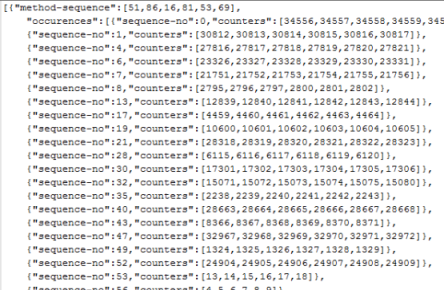
\includegraphics{shortestsubsequence}
\caption{Results of one of the thresholds for Shortest SubSequence.}
\label{shortestsubsequence}
\end{figure}

\section{Settings.java}
\lstset{language=Java, caption=Settings.java, label=DescriptiveLabel,breaklines=true,breakatwhitespace=false,keywordstyle=\color{blue},identifierstyle=\color{black},commentstyle=\color{green}}
\lstinputlisting{Settings.java}

\section{MyTest.java}
\lstset{language=Java, caption=MyTest.java, label=DescriptiveLabel,breaklines=true,breakatwhitespace=false,keywordstyle=\color{blue},identifierstyle=\color{black},commentstyle=\color{green}}
\lstinputlisting{abcd.java}